\documentclass[a4paper]{article}

%====================== PACKAGES ======================

\usepackage[french]{babel}
\usepackage[utf8x]{inputenc}
\usepackage{float}
\usepackage{amsmath}
\usepackage{graphicx}
\usepackage[colorinlistoftodos]{todonotes}
\usepackage{url}
\usepackage{hyperref}
\usepackage{array}
\usepackage{tabularx}
\usepackage{setspace}
\usepackage{abstract}
\usepackage[T1]{fontenc}
\usepackage[top=2cm, bottom=2cm, left=2cm, right=2cm]{geometry}
\usepackage{subfig}
\usepackage{listings}
\usepackage{xcolor}
\usepackage{adjustbox}

%====================== CUSTOM SETTINGS ======================
\lstset{
  basicstyle=\ttfamily\footnotesize,
  breaklines=true,
  frame=single,
  numberstyle=\tiny,
  keywordstyle=\color{blue},
  commentstyle=\color{gray},
  stringstyle=\color{red},
  showstringspaces=false
}

\lstdefinelanguage{JavaScript}{
  keywords={typeof, new, true, false, catch, function, return, null, catch, switch, var, if, in, while, do, else, case, break},
  keywordstyle=\color{blue}\bfseries,
  ndkeywords={class, export, boolean, throw, implements, import, this},
  ndkeywordstyle=\color{darkgray}\bfseries,
  identifierstyle=\color{black},
  sensitive=false,
  comment=[l]{//},
  morecomment=[s]{/*}{*/},
  commentstyle=\color{purple}\ttfamily,
  stringstyle=\color{red}\ttfamily,
  morestring=[b]',
  morestring=[b]"
}


% Numérotation des sections et sous-sections
\setcounter{secnumdepth}{4}
\setcounter{tocdepth}{4}

%======================== DEBUT DU DOCUMENT ========================

\begin{document}

% Commande pour la ligne horizontale
\newcommand{\HRule}{\rule{\linewidth}{0.5mm}}

%=========================== PAGE DE GARDE ===========================

\begin{center}
% Haut de la page

\includegraphics[width=0.35\textwidth]{./logo}~\\[2cm]
\vspace{3cm}
% Titre
\textsc{\LARGE INSA Lyon}\\[0.5cm]
\textsc{\Large Département Informatique}\\[0.5cm]
\HRule \\[0.4cm]
{\huge \bfseries Projet Web Sémantique\\
Spezialsuchmaschine\\[0.4cm] }
\HRule \\[1.5cm]
% Auteurs et encadrants
\begin{minipage}{0.4\textwidth}
\begin{flushleft} \large
\emph{Auteurs:} \\
Hazim \textsc{Asri}\\
Nihal \textsc{Boutadghart}\\
Malte \textsc{Camier}\\
Jassir \textsc{Habba}\\
Junior \textsc{Noukam}\\
Simon \textsc{Perret}\\
\end{flushleft}
\end{minipage}
\begin{minipage}{0.4\textwidth}
\begin{flushright} \large
\emph{Encadrants:} \\
M. \textsc{Bento}\\
Mme. \textsc{Calabretto}\\
\end{flushright}
\end{minipage}
\vfill
% Bas de la page
{\large \today}
\end{center}

%======================== TABLE DES MATIERES ========================
\newpage
\tableofcontents
\newpage

%====================== CONTENU DU RAPPORT ======================

% Introduction
\section{Introduction}
Le développement des technologies du Web Sémantique a permis une avancée majeure dans la manière dont les données sont connectées, interprétées et exploitées sur le web. Contrairement au Web traditionnel, le Web Sémantique repose sur des structures standardisées et interopérables qui permettent une meilleure compréhension des données par les machines. À travers ce projet, nous avons exploré ces technologies en concevant une application de recherche spécialisée, exploitant les concepts de données liées et les requêtes SPARQL. \\

\noindent
\textbf{Objectif principal :}
Créer un moteur de recherche interactif et intuitif, capable d'explorer un domaine spécifique – celui des marques automobiles allemandes et de leurs modèles – à partir des données RDF disponibles sur DBpedia. \\

\noindent
\textbf{Enjeux majeurs du projet :}
\begin{itemize}
    \item \textbf{Exploitation des données structurées :} Manipuler des données hétérogènes, mais interconnectées, en utilisant des outils adaptés comme SPARQL pour les interroger.
    \item \textbf{Accessibilité et visualisation :} Rendre ces données accessibles à l'utilisateur final à travers une interface claire, ergonomique et interactive.
    \item \textbf{Défis technologiques :} Relever les défis liés à la dépendance envers DBpedia, à la complexité des requêtes SPARQL et à l'intégration des résultats dans une application moderne.
\end{itemize}

Ce projet ne se limite pas à une simple implémentation technique ; il offre également une réflexion sur les avantages et les limites des technologies du Web Sémantique dans le cadre d'une application concrète. Le rapport qui suit détaille les aspects techniques, les fonctionnalités implémentées, ainsi que les défis rencontrés et les apprentissages réalisés.

% Technologies et outils utilisés
\section{Technologies et Outils Utilisés}
\subsection{Technologies Principales}
\begin{itemize}
    \item \textbf{SPARQL} : Langage de requête pour les bases de données RDF.
    \item \textbf{DBpedia} : Base de données sémantique utilisée pour les marques automobiles.
    \item \textbf{HTML/CSS} : Structure et design de l'interface utilisateur.
    \item \textbf{JavaScript} : Interaction dynamique avec les utilisateurs et génération de requêtes SPARQL.
\end{itemize}

\subsection{Outils de Développement}
\begin{itemize}
    \item \textbf{Visual Studio Code} : IDE principal pour le développement.
    \item \textbf{GitHub} : Gestion de version pour la collaboration.
    \item \textbf{Firefox} : Débogage et optimisation de l'application.
\end{itemize}

\newpage

% Architecture et fonctionnement
\section{Architecture et Fonctionnement}
\subsection{Organisation des Fichiers}
Le projet est structuré de manière logique pour séparer le code, le style et les fonctionnalités. Voici l'organisation :
\begin{verbatim}
/-- docs/
    /-- presentation/
        /-- images/
            |-- ...
        |-- main.tex
        |-- main.pdf
        |-- logo.png
    /-- report/
        /-- images/
            |-- ...
        |-- main.tex
        |-- main.pdf
        |-- logo.png
/-- images/
    |-- favicon.ico
/-- scripts/
    |-- marque.js
    |-- marques.js
    |-- modele.js
    |-- recherche.js
    |-- requetes.js
/-- styles/
    |-- index.css
    |-- main.css
    |-- marque.css
    |-- modele.css
    |-- recherche.css
/-- index.html
/-- marque.html
/-- marques.html
/-- modele.html
/-- README.md
\end{verbatim}

\subsection{Organisation des Fichiers}
\begin{itemize}
    \item \textbf{docs/} : Contient les rapports et présentations.
    \item \textbf{images/} : Images utilisées dans l'application.
    \item \textbf{scripts/} : Scripts JavaScript pour chaque page.
    \item \textbf{styles/} : Feuilles de style CSS pour chaque page.
    \item \textbf{index.html} : Page d'accueil de l'application.
    \item \textbf{marque.html} : Page détaillée d'une marque.
    \item \textbf{marques.html} : Liste des marques automobiles allemandes.
    \item \textbf{modele.html} : Page détaillée d'un modèle de voiture.
    \item \textbf{README.md} : Description du projet et instructions
\end{itemize}

\subsection{Flux de Données}
\begin{itemize}
    \item L'utilisateur interagit avec l'interface en entrant un mot-clé dans la barre de recherche.
    \item Le mot-clé saisi est traité par un script JavaScript, qui construit dynamiquement une requête SPARQL adaptée au contexte (recherche de marques, de modèles, ou de détails spécifiques).
    \item La requête SPARQL est envoyée à l'endpoint public de DBpedia via une requête HTTP.
    \item Les résultats au format JSON sont analysés et traités pour extraire les informations pertinentes (noms, descriptions, images, etc.).
    \item Les données sont intégrées à l'interface sous forme de cartes interactives, permettant à l'utilisateur de visualiser et de naviguer facilement parmi les résultats.
\end{itemize}
% Fonctionnalités
\section{Fonctionnalités}
Le choix du sujet a été une étape cruciale dans notre projet. Nous avons voulu nous concentrer sur un domaine à la fois captivant et structuré, afin de pouvoir exploiter pleinement les liens sémantiques entre les données. Nous avons en premier temps opté pour un moteur de recherche sur les voitures en générale, cependant nous avons dans notre groupe un étudiant Erasmus venant d'Allemagne, nous avons finalement choisi le thème des automobiles allemandes. DBpedia, avec ses données bien organisées, nous a permis de tisser des connexions entre les modèles, les marques, et leurs caractéristiques respectives. \\ 

Nos fonctionnalités incluent les éléments suivants : pour chaque marque, nous affichons son nom, son logo, sa date de fondation et un lien vers son site officiel. Concernant les modèles, nous fournissons une description détaillée, l'année de production, le type de moteur, le design et des images illustrant chaque véhicule. Ces informations sont présentées sous forme de cartes interactives, offrant une navigation claire et intuitive. \\

Pour rendre l'expérience utilisateur plus fluide, nous avons intégré une barre de recherche avec une auto-complétion qui permet de saisir facilement le nom d'une marque ou d'un modèle. Cette fonctionnalité guide également l'utilisateur en proposant des suggestions pertinentes, même en cas de saisie partielle. De plus, nous avons implémenté une normalisation des chaînes de caractères pour éviter les erreurs dues à la casse, permettant ainsi une recherche sans contrainte sur la forme du texte. \\

Enfin, notre application organise les marques de manière alphabétique, offrant une vue d'ensemble intuitive et un accès rapide aux informations. Cette approche exploite pleinement les données sémantiques pour offrir une expérience enrichissante et interactive à l'utilisateur.

\subsection{Recherche Interactive}
La recherche interactive permet à l'utilisateur de rechercher des marques et des modèles automobiles allemands en temps réel. Les résultats sont affichés sous forme de pages interactives, avec des images et des informations détaillées.

\begin{figure}[H]
    \centering
    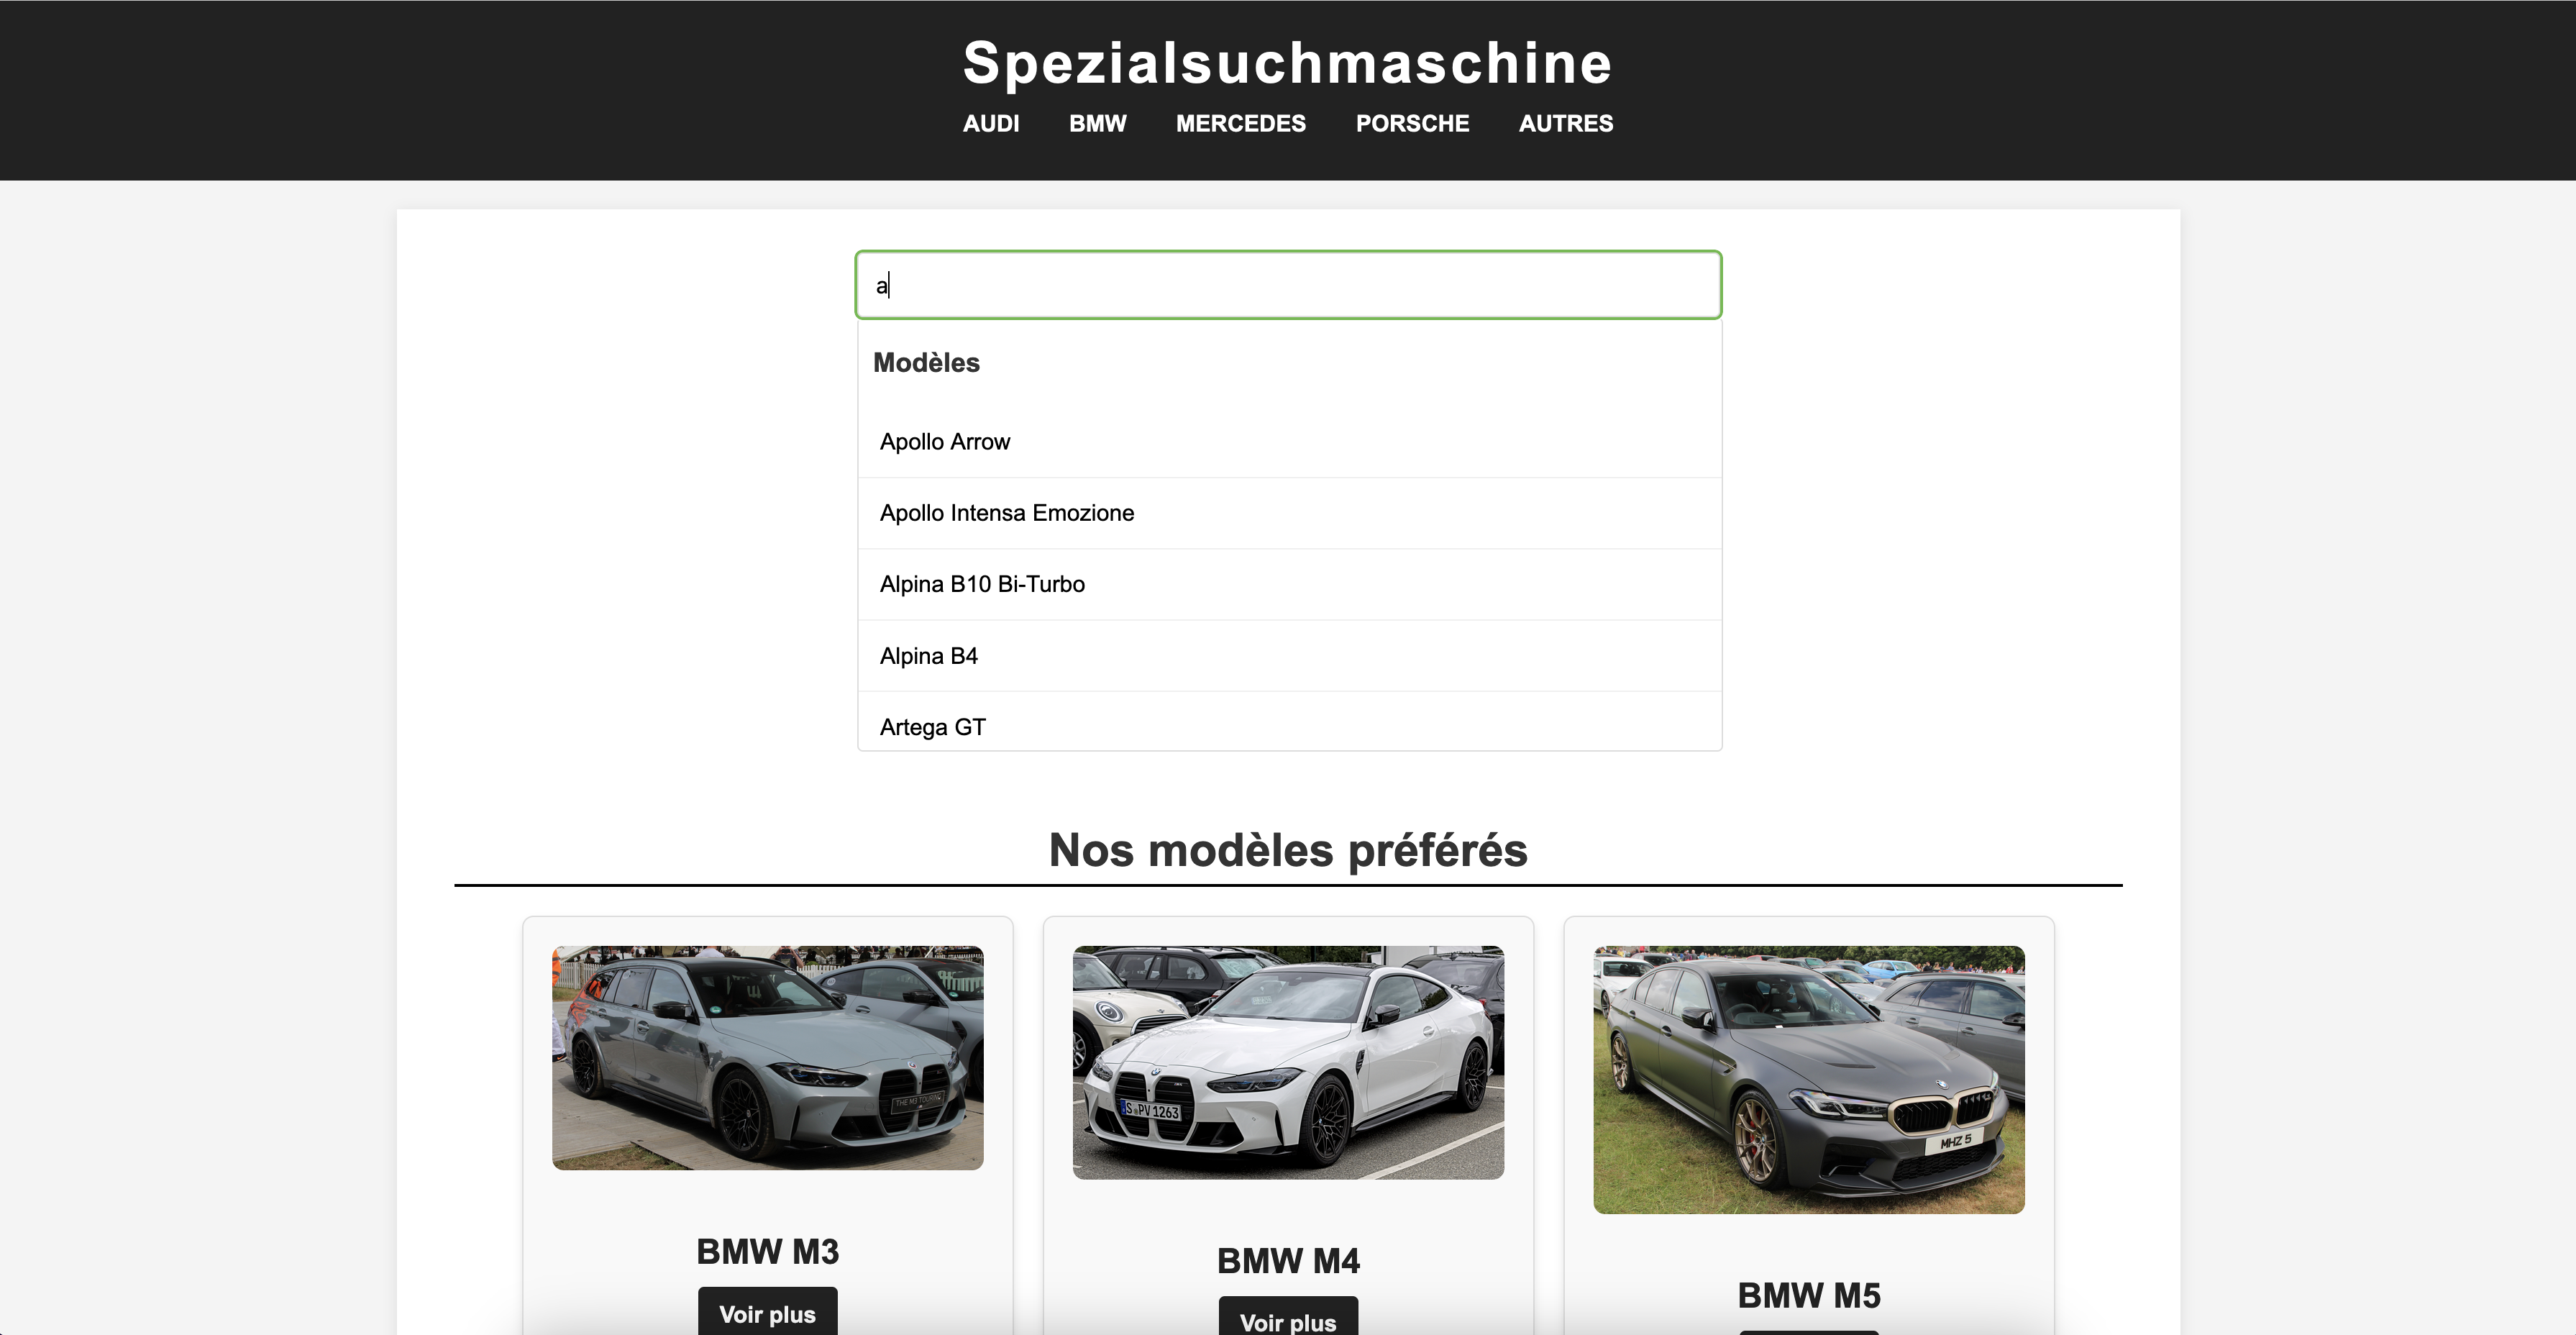
\includegraphics[width=0.8\textwidth]{images/recherche.png}
    \caption{Recherche interactive de marques et modèles}
\end{figure}

\begin{lstlisting}[language=SPARQL, caption=Requête SPARQL pour rechercher une marques allemandes]
    SELECT DISTINCT ?model ?modelLabel ?manufacturer ?manufacturerLabel
    WHERE {
        ?manufacturer dct:subject dbc:Car_manufacturers_of_Germany .
    
        ?model (dbo:manufacturer|dbp:manufacturer) ?manufacturer .
        ?model rdf:type dbo:Automobile .
    
        ?model rdfs:label ?modelLabel .
        FILTER(LANG(?modelLabel) = "fr") .
        ?manufacturer rdfs:label ?manufacturerLabel .
        FILTER(LANG(?manufacturerLabel) = "fr") .
        FILTER(REGEX(STR(?modelLabel), "^a", "i")) .
    }
    LIMIT 5
\end{lstlisting}

\begin{lstlisting}[language=SPARQL, caption=Requête SPARQL pour rechercher un modèle allemand]
    SELECT DISTINCT ?manufacturer ?manufacturerLabel 
    WHERE {
        ?manufacturer dct:subject dbc:Car_manufacturers_of_Germany .
        ?manufacturer rdfs:label ?manufacturerLabel .
        FILTER(LANG(?manufacturerLabel) = "en") .
        FILTER(REGEX(STR(?manufacturerLabel), "^a", "i")) .
    }
    ORDER BY ASC(?manufacturerLabel) 
    LIMIT 5
\end{lstlisting}

\subsection{Affichage des Marques}
\begin{itemize}
    \item Liste des marques allemandes triées par ordre alphabétique.
    \item Possibilité de cliquer sur la marque pour obtenir plus d'informations.
\end{itemize}

\begin{figure}[H]
    \centering
    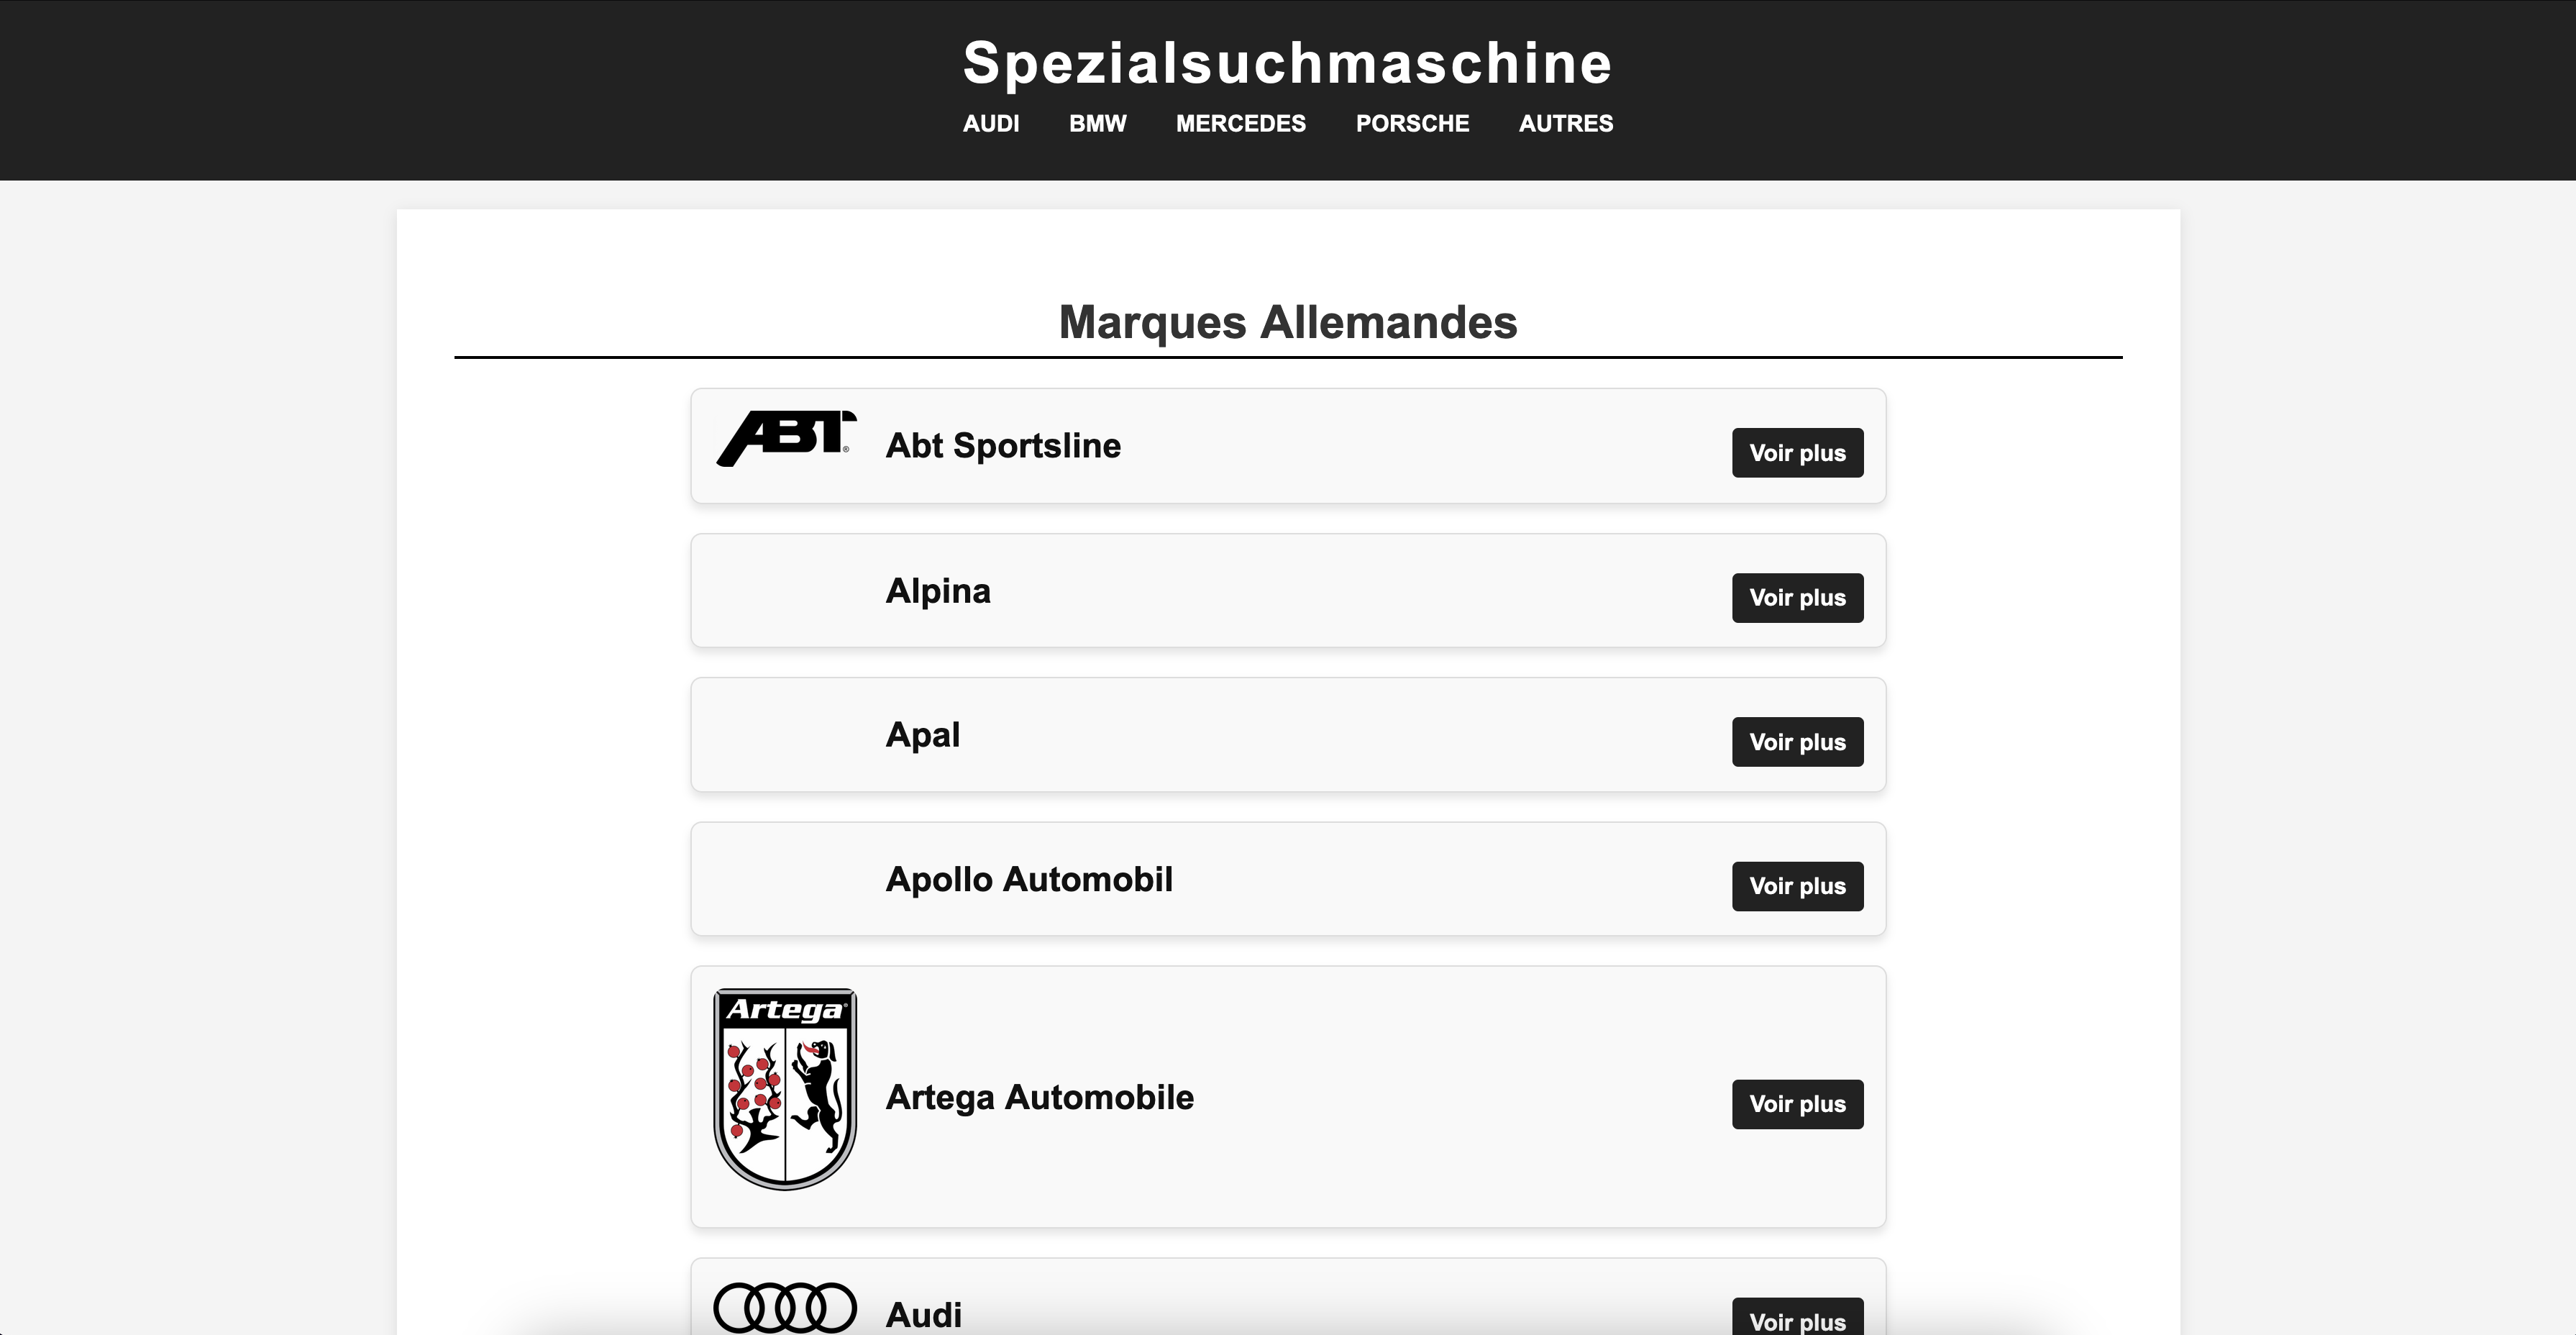
\includegraphics[width=0.8\textwidth]{images/marques.png}
    \caption{Liste des marques automobiles allemandes}
\end{figure}

\begin{lstlisting}[language=SPARQL, caption=Requête SPARQL pour rechercher toutes les marques allemandes]
    PREFIX dbo: <http://dbpedia.org/ontology/>
    PREFIX dbc: <http://dbpedia.org/resource/Category:>
    PREFIX rdfs: <http://www.w3.org/2000/01/rdf-schema#>
    PREFIX dct: <http://purl.org/dc/terms/>

    SELECT DISTINCT ?manufacturer ?manufacturerLabel ?thumbnail
    WHERE {
        ?manufacturer dct:subject dbc:Car_manufacturers_of_Germany .
        ?manufacturer rdfs:label ?manufacturerLabel .
        FILTER(LANG(?manufacturerLabel) = "en") .
        ?manufacturer dbo:thumbnail ?thumbnail
    }
    ORDER BY ASC(?manufacturerLabel)
\end{lstlisting}

\subsection{Affichage d'une marque}
\begin{itemize}
    \item Informations détaillées : description, site web, année de fondation, etc.
    \item Images pour illustrer chaque marque.
    \item Lorsque les informations sont manquantes, le container est rendu invisible.
    \item Nous avons fait le choix de rendre chaques requêtes indépendantes pour éviter les erreurs de chargement.
\end{itemize}
\begin{figure}[H]
    \centering
    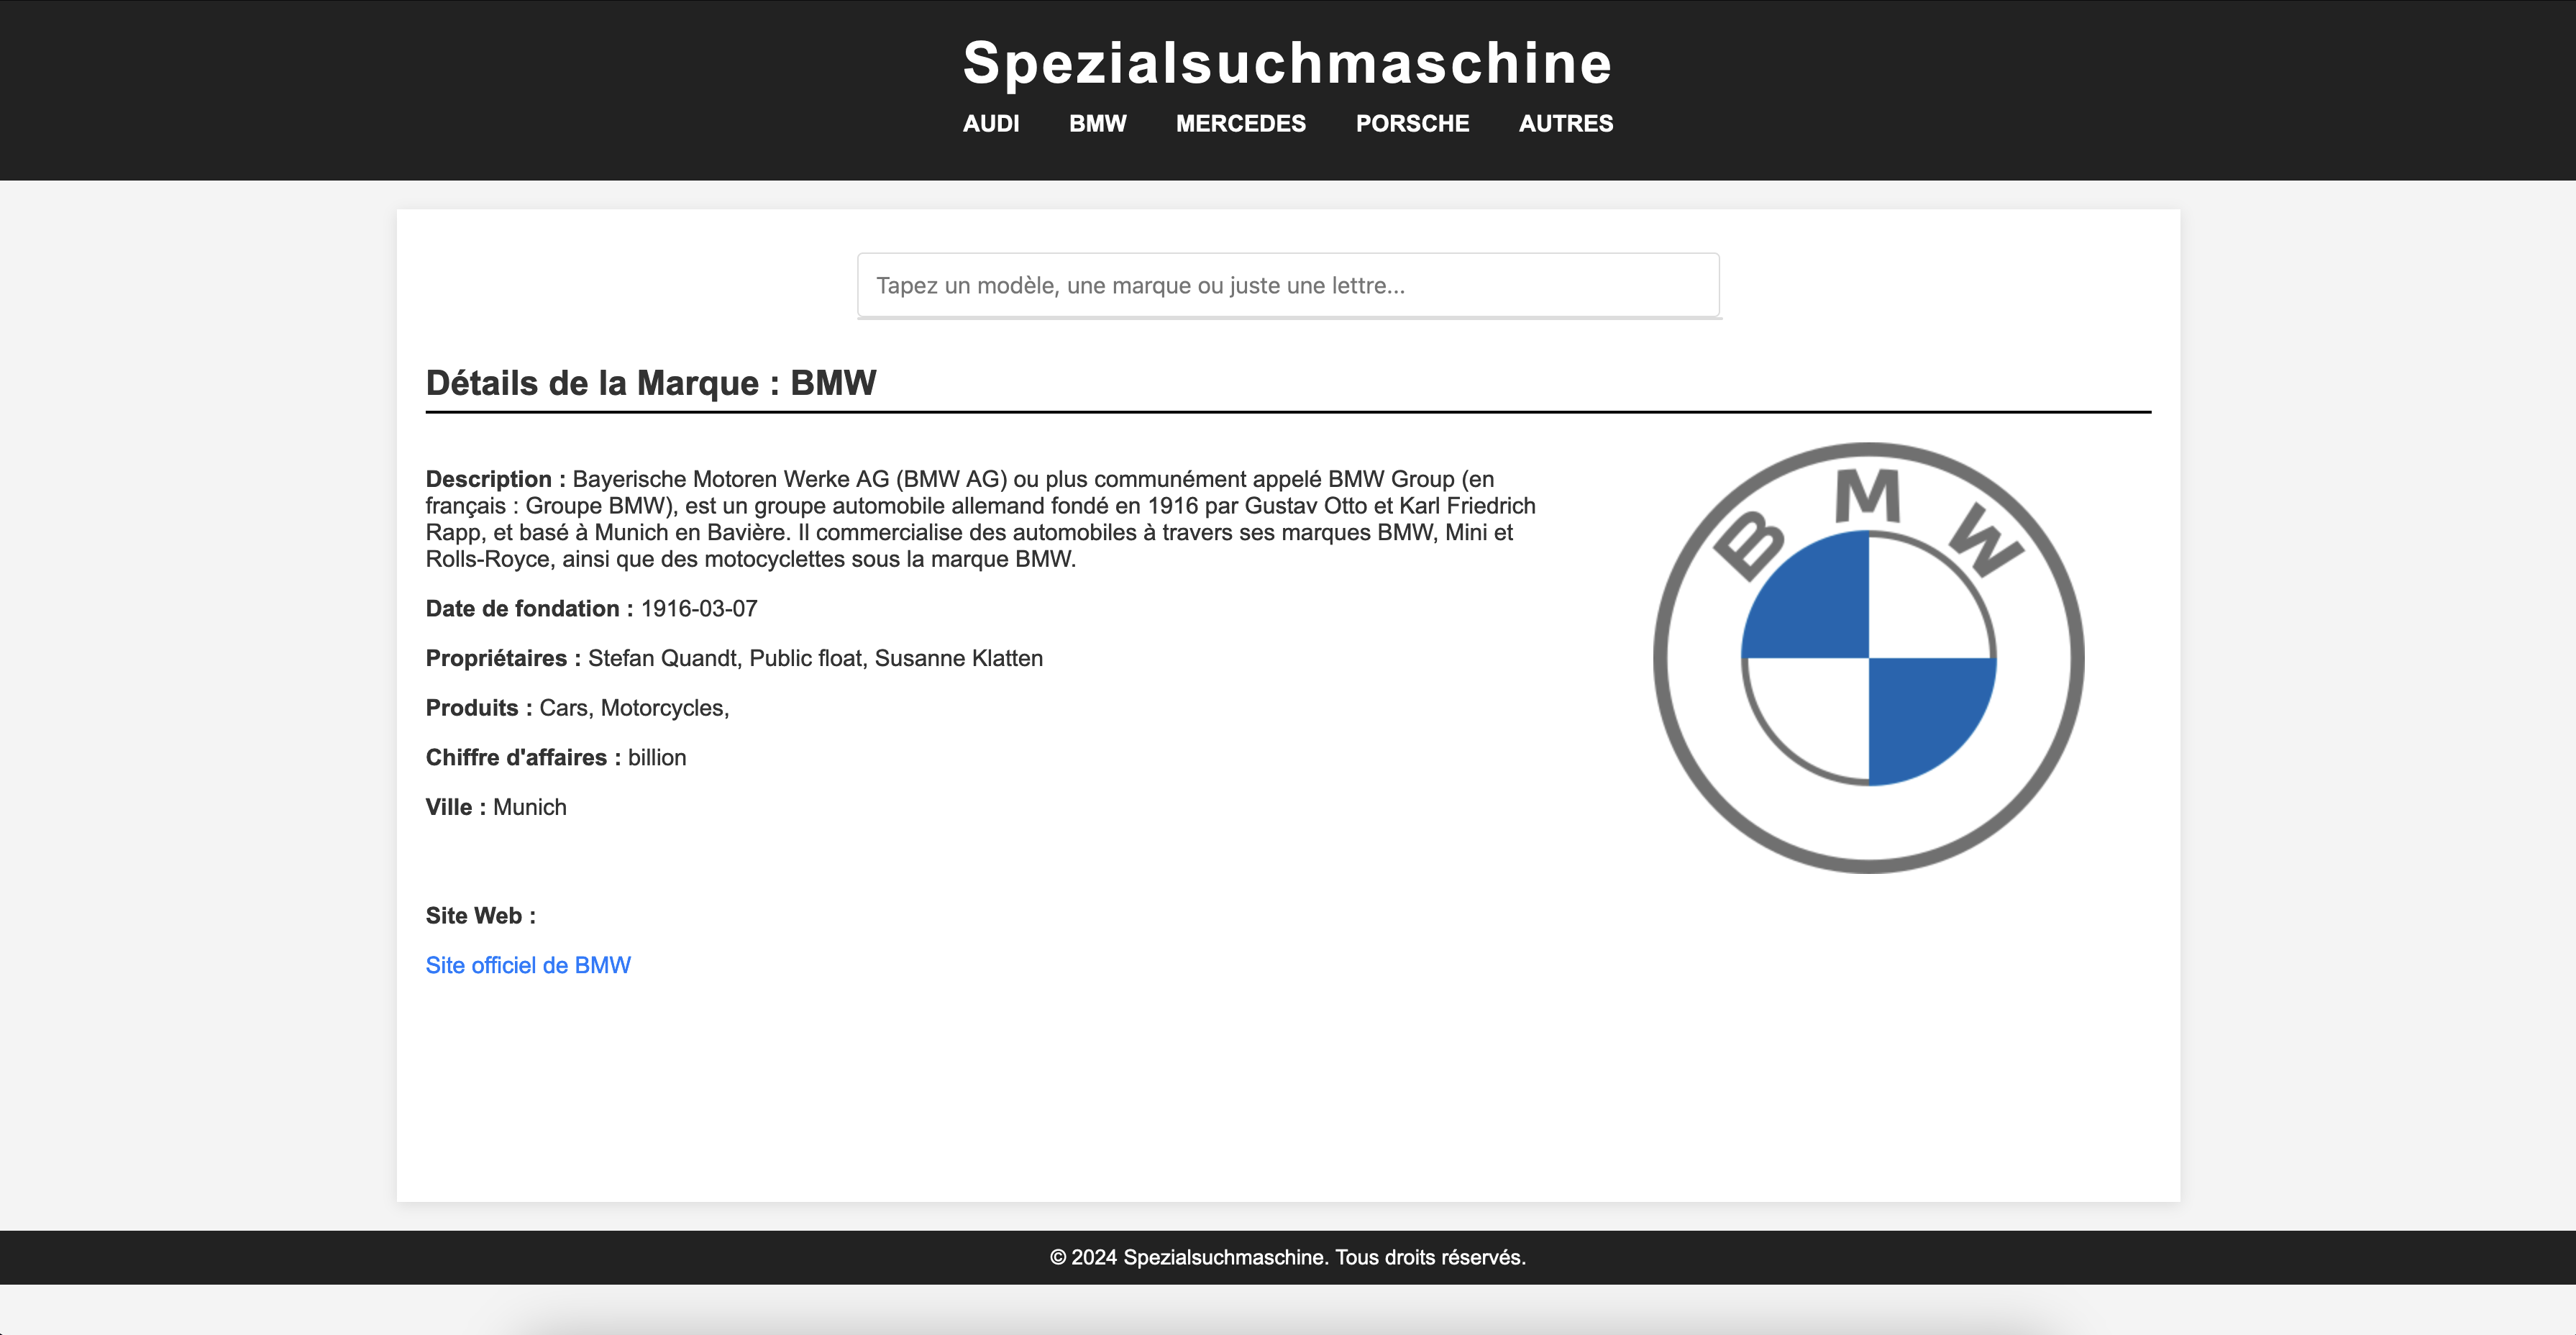
\includegraphics[width=0.8\textwidth]{images/marque.png}
    \caption{Affichage des détails d'une marque}
\end{figure}

\begin{lstlisting}[language=SPARQL, caption=Requêtes SPARQL pour rechercher la ville d'une marque]
    SELECT DISTINCT ?locationCity ?locationCityName
    WHERE {
    OPTIONAL {
        <http://dbpedia.org/resource/BMW> dbp:locationCity ?locationCity .
        ?locationCity rdfs:label ?locationCityName .
        FILTER(LANG(?locationCityName) = "en") .
        }
        OPTIONAL {
        <http://dbpedia.org/resource/BMW> dbo:location ?locationCity .
        ?locationCity rdfs:label ?locationCityName .
        FILTER(LANG(?locationCityName) = "en") .
        }
    }
\end{lstlisting}

\subsection{Affichage des Modèles}
\begin{itemize}
    \item Informations détaillées : description, moteur, année de production, etc.
    \item Images pour illustrer chaque modèle.
    \item Lorsque les informations sont manquantes, le container est rendu invisible (idem que pour les marques)
\end{itemize}

\begin{figure}[H]
    \centering
    % \includegraphics[width=0.8\textwidth]{capture_interface.png}
    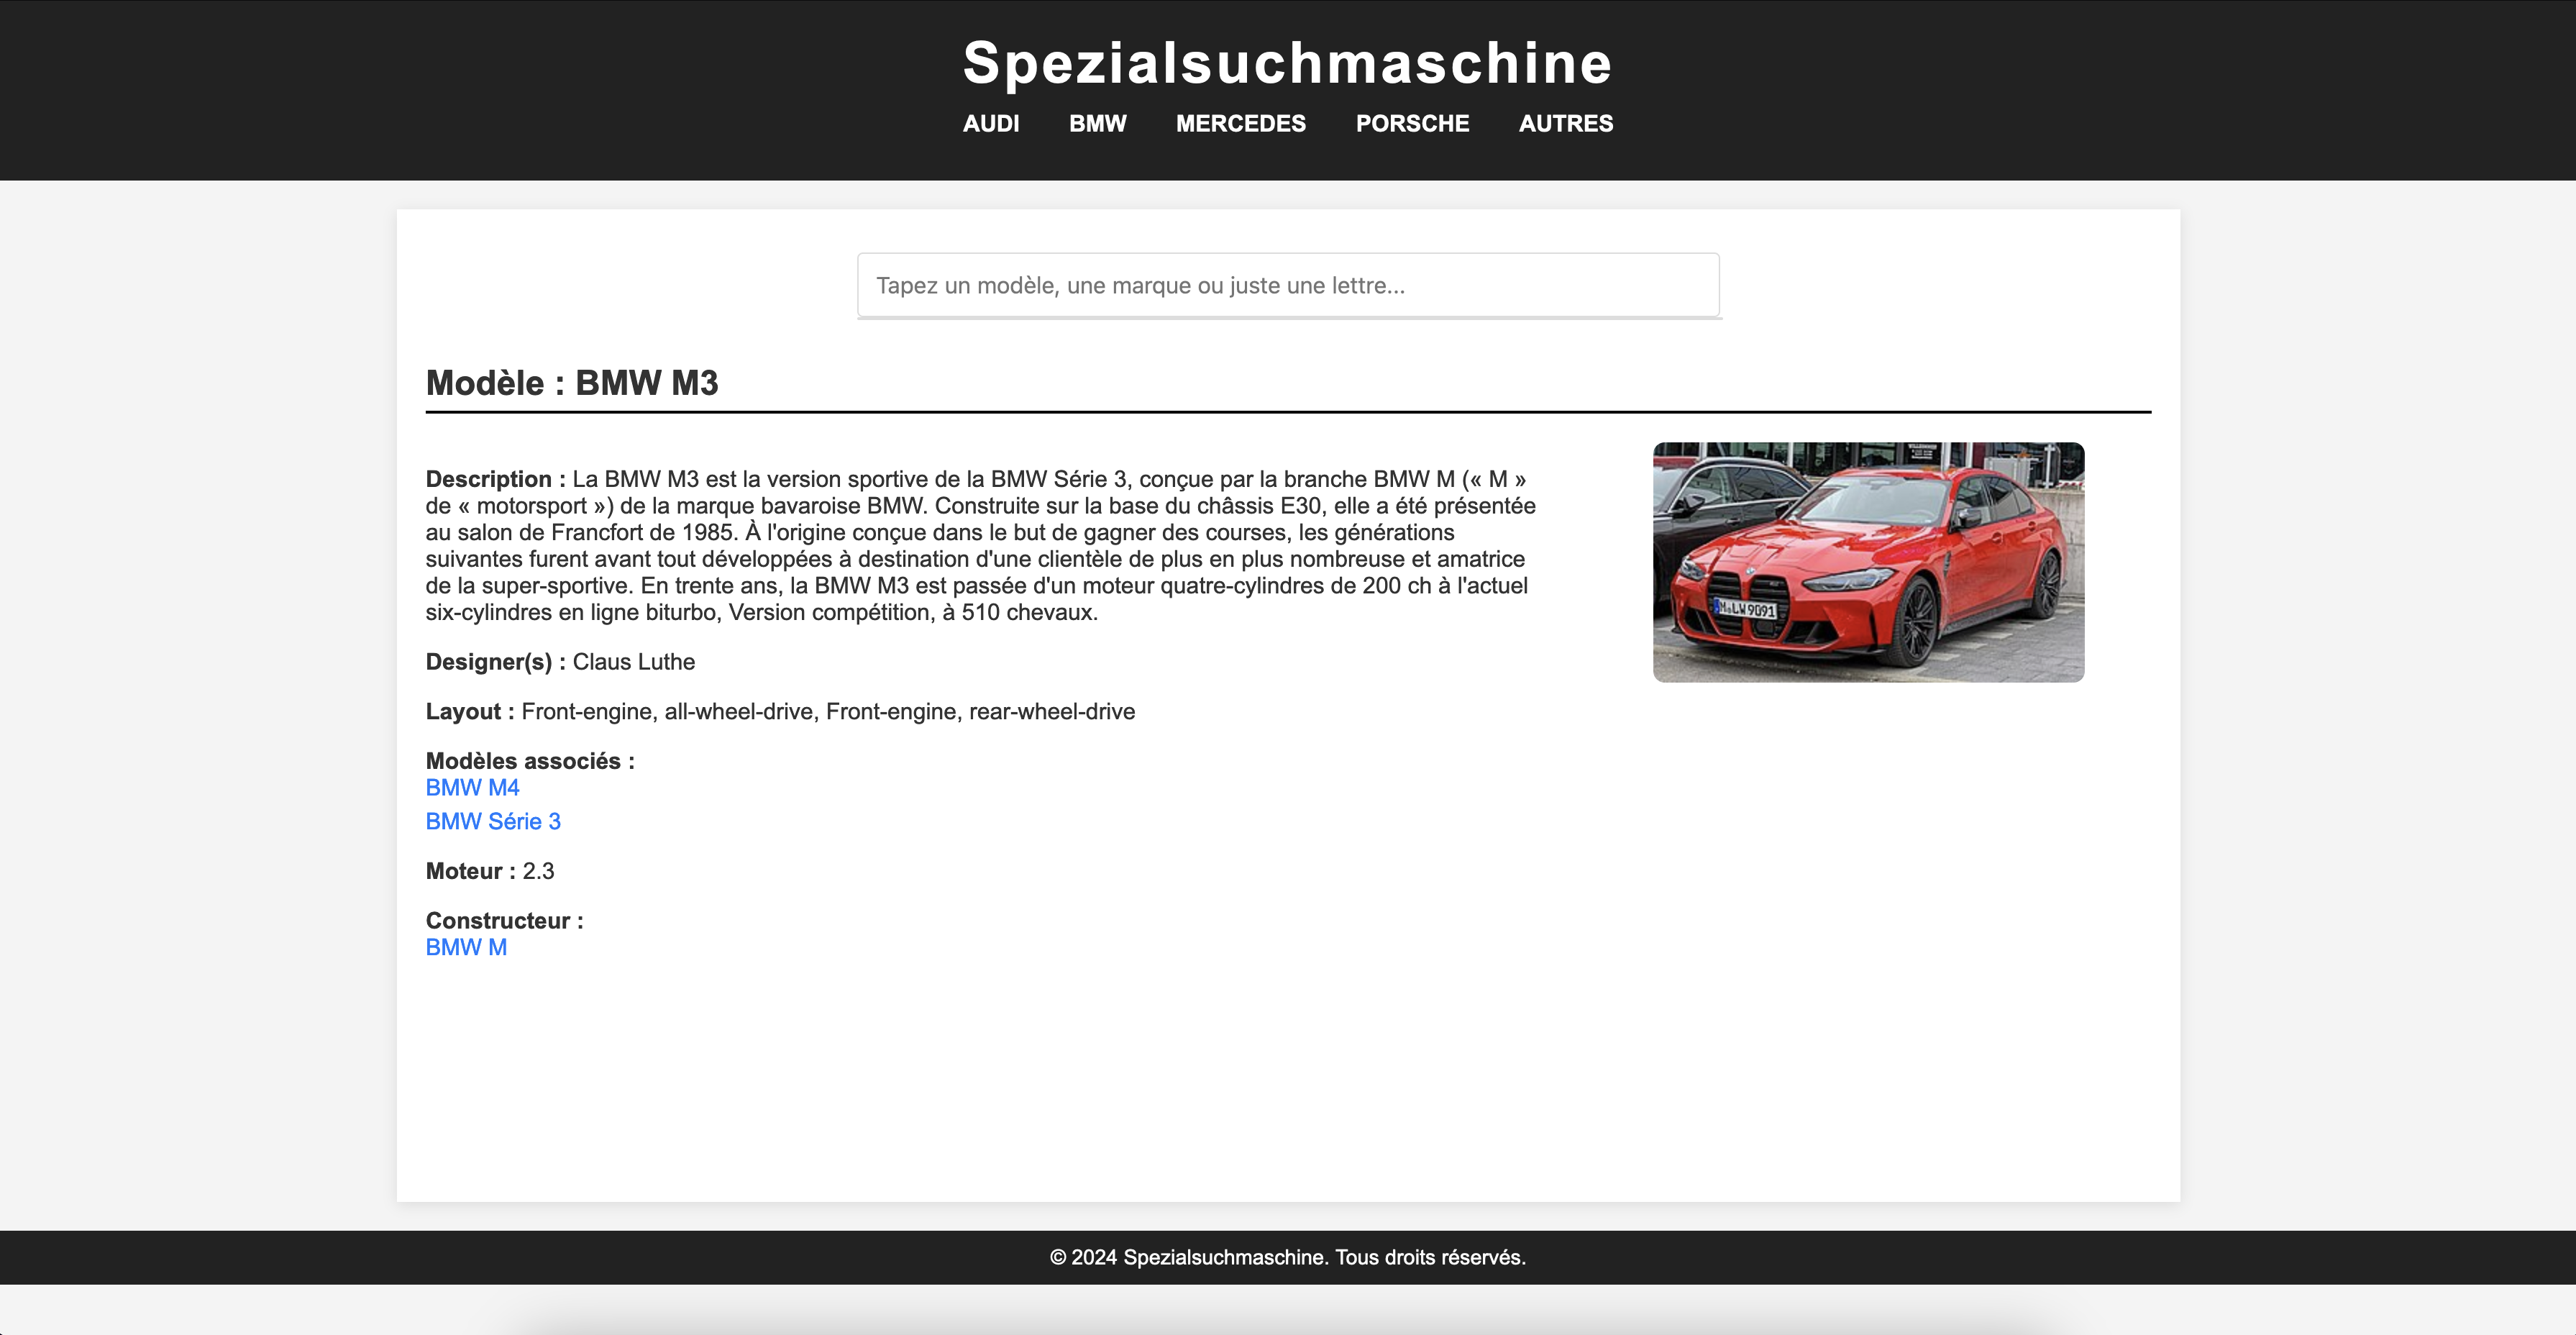
\includegraphics[width=0.8\textwidth]{images/modele.png}
    \caption{Affichage des détails d'un modèle}
\end{figure}

\begin{lstlisting}[language=SPARQL, caption=Requêtes SPARQL pour rechercher la configuration d'un modèle]
    SELECT DISTINCT ?layoutLabel
    WHERE {
    OPTIONAL {
        <http://dbpedia.org/resource/BMW_M3> dbp:layout ?layout .
        ?layout rdfs:label ?layoutLabel .
        FILTER(LANG(?layoutLabel) = "en") .
        }
    }
\end{lstlisting}

\section{Réflexion sur le Web Sémantique}

Le Web Sémantique représente une évolution majeure du web, visant à rendre les données non seulement accessibles, mais aussi compréhensibles par les machines. À travers ce projet, nous avons pu constater à la fois les avantages et les défis liés à l'utilisation de ces technologies pour la construction d'un moteur de recherche spécialisé. Voici une réflexion sur ces aspects.

\subsection{Avantages du Web Sémantique}

\paragraph{Interconnexion des données} L'un des principaux atouts du Web Sémantique est l'interconnexion des données, permettant à des informations provenant de sources diverses d'être intégrées et exploitées ensemble. Dans notre projet, l'utilisation de DBpedia comme source de données RDF a permis de lier de manière transparente des informations sur les marques, les modèles de voitures et leurs caractéristiques, créant ainsi un réseau riche et structuré de données liées.

\paragraph{Interopérabilité et Flexibilité} Grâce aux standards ouverts comme RDF, SPARQL et OWL, le Web Sémantique offre une interopérabilité entre différents systèmes, indépendamment de leur plateforme ou de leur technologie sous-jacente. Ce projet a démontré la puissance de ces standards pour interroger et manipuler des bases de données distribuées et hétérogènes. Par exemple, les requêtes SPARQL que nous avons utilisées permettent de récupérer des informations très spécifiques tout en étant flexibles quant aux données recherchées.

\paragraph{Amélioration de la recherche} Le Web Sémantique permet une recherche plus précise et intelligente grâce à l'exploitation des métadonnées et des ontologies. L'utilisation de SPARQL permet de poser des requêtes complexes qui vont au-delà des simples recherches par mots-clés. L'intégration de filtres linguistiques et de correspondances partielles dans les requêtes a facilité la recherche de marques et de modèles, ce qui est un pas en avant par rapport aux moteurs de recherche traditionnels.

\subsection{Limites et Défis du Web Sémantique}

\paragraph{Complexité de l'intégration} L'un des défis majeurs rencontrés dans le cadre de ce projet a été l'intégration des données RDF dans une application web traditionnelle. Bien que le Web Sémantique propose une structure de données très puissante, il nécessite des connaissances spécifiques, notamment sur la modélisation RDF, la formulation de requêtes SPARQL et l'exploitation des ontologies. De plus, les résultats obtenus sont parfois complexes à manipuler et à afficher dans une interface utilisateur classique.

\paragraph{Performance et Scalabilité} L'un des inconvénients évidents du Web Sémantique est la performance, surtout lorsque les requêtes deviennent plus complexes ou que la taille des données augmente. L'interrogation de grandes bases de données via SPARQL peut être lente, notamment si l'on travaille avec des endpoints publics comme DBpedia. Dans un contexte de production, il serait nécessaire d'optimiser les performances pour éviter les latences et garantir une expérience utilisateur fluide.

\paragraph{Dépendance aux sources externes} Notre projet s'appuie sur DBpedia pour obtenir des données sur les marques et les modèles automobiles. Cette dépendance à une source externe a soulevé des questions liées à la fiabilité, la mise à jour des données, et la disponibilité du service. Le Web Sémantique repose sur la disponibilité et la qualité des données de source ouverte, ce qui peut poser problème si ces données deviennent obsolètes ou si les services d'accès ne sont plus disponibles.

\subsection{Enseignements tirés du projet}

\paragraph{Importance de la modélisation des données} Ce projet a mis en lumière l'importance d'une bonne modélisation des données pour tirer pleinement parti des avantages du Web Sémantique. Bien que DBpedia offre une riche base de connaissances, une modélisation propre et une utilisation adéquate des ontologies peuvent permettre de construire des applications beaucoup plus puissantes, capables de raisonner sur les données et de les connecter de manière plus intelligente.

\paragraph{L'expérience utilisateur} Il est également important de noter que l'expérience utilisateur joue un rôle crucial dans l'acceptation de technologies comme le Web Sémantique. Bien que les données sémantiques puissent être extrêmement riches, elles ne sont utiles que si elles sont accessibles de manière intuitive et pratique pour l'utilisateur. Ce projet a permis de mieux comprendre les défis liés à la conception d'interfaces utilisateur pour des applications sémantiques, en mettant l'accent sur la simplicité et l'interactivité.

\paragraph{Potentiel d'évolutivité} Enfin, ce projet a montré que le Web Sémantique offre un énorme potentiel pour l'évolutivité des applications. En exploitant des données ouvertes et liées, il est possible de faire évoluer l'application pour inclure de nouveaux domaines ou de nouvelles sources de données sans devoir réécrire l'ensemble de l'infrastructure. L'application pourrait facilement être adaptée pour intégrer d'autres secteurs ou d'autres types de données en utilisant les mêmes principes de base.

\subsection{Conclusion} Le Web Sémantique offre de nombreuses opportunités pour améliorer la recherche et la gestion des données sur le web. Cependant, sa mise en œuvre dans des applications concrètes nécessite une prise en compte des défis techniques et des exigences spécifiques liées à la manipulation de données liées. Ce projet nous a permis de mieux comprendre l'importance de la structuration des données, des requêtes complexes, et de l'interaction entre les utilisateurs et les données sémantiques.


\section{Conclusion}
Ce projet a permis d'explorer et d'appliquer les technologies du Web Sémantique dans le cadre de la création d'un moteur de recherche spécialisé. À travers l'utilisation des données RDF et des requêtes SPARQL, nous avons pu concevoir une application interactive permettant d'explorer les marques et modèles automobiles allemands, avec une interface utilisateur claire et intuitive. \\

Les technologies et outils employés, tels que DBpedia et SPARQL, ont joué un rôle essentiel dans la manipulation des données structurées, offrant une vue d'ensemble enrichissante et détaillée des informations. Le principal défi résidait dans l'intégration fluide de ces données sémantiques au sein d'une interface web moderne, ce que nous avons réussi à réaliser avec succès. \\

En conclusion, ce projet a non seulement renforcé nos compétences techniques en développement web et en Web Sémantique, mais a également montré l'énorme potentiel de ces technologies pour offrir des solutions intelligentes et performantes dans la gestion de données complexes et interconnectées. Nous espérons que cette application pourra servir de modèle pour d'autres domaines d'application, et que l'exploration du Web Sémantique continuera à évoluer pour enrichir davantage nos interactions avec les données sur le web.


\end{document}
